\documentclass{article}
\usepackage{tikz}
\usepackage{pgfplots}
\usepackage{svg}
\usepackage{amsmath}
\usepackage{array}
\usepackage[skins]{tcolorbox}
\usepackage[version=4]{mhchem}
\usepackage[a4paper, total={6in, 9in}]{geometry}
\usepackage{fourier}
\usepackage{xymtex}
\usepackage{textcomp}
\usepackage{eurosym}
\usepackage{caption}
\usepackage{longtable}
\usepackage{float}
\usepackage{attachfile}
\usepackage{multirow}
\usepackage{amsfonts} 
\usepackage{xcolor}
\usepackage{tabularray}
\UseTblrLibrary{booktabs}

\captionsetup[table]{name=\textit{Tabella}}
\pagenumbering{gobble}
%\setcounter{secnumdepth}{2}

\definecolor{myblue}{RGB}{224, 245, 255} 
\definecolor{myred}{RGB}{234, 222, 255}
\definecolor{myorange}{RGB}{255, 102, 0}

\renewcommand*\contentsname{Indice}
\setcounter{tocdepth}{3}
\setcounter{secnumdepth}{2}
\pgfplotsset{compat=1.15}


\title{Relazione di laboratorio - Esperienza di Poisson}
\author{Federico Cesari}
\date{Marzo 2024}




\begin{document}
\begin{titlepage}
	\begin{center}
		\vspace*{1cm}
		
		\textbf{\LARGE Relazione di laboratorio - Pendolo semplice}
		
		\vspace{0.3cm}
		\large \textit{Misura del periodo di un pendolo semplice} \\
		
		\vspace{0.5cm}
		\Large Federico Cesari \\
		
		\small 1096759 
		\vspace{0.2cm}
		
		\small Gruppo 5
		
		
		\vspace{3cm}
		\begin{center}
			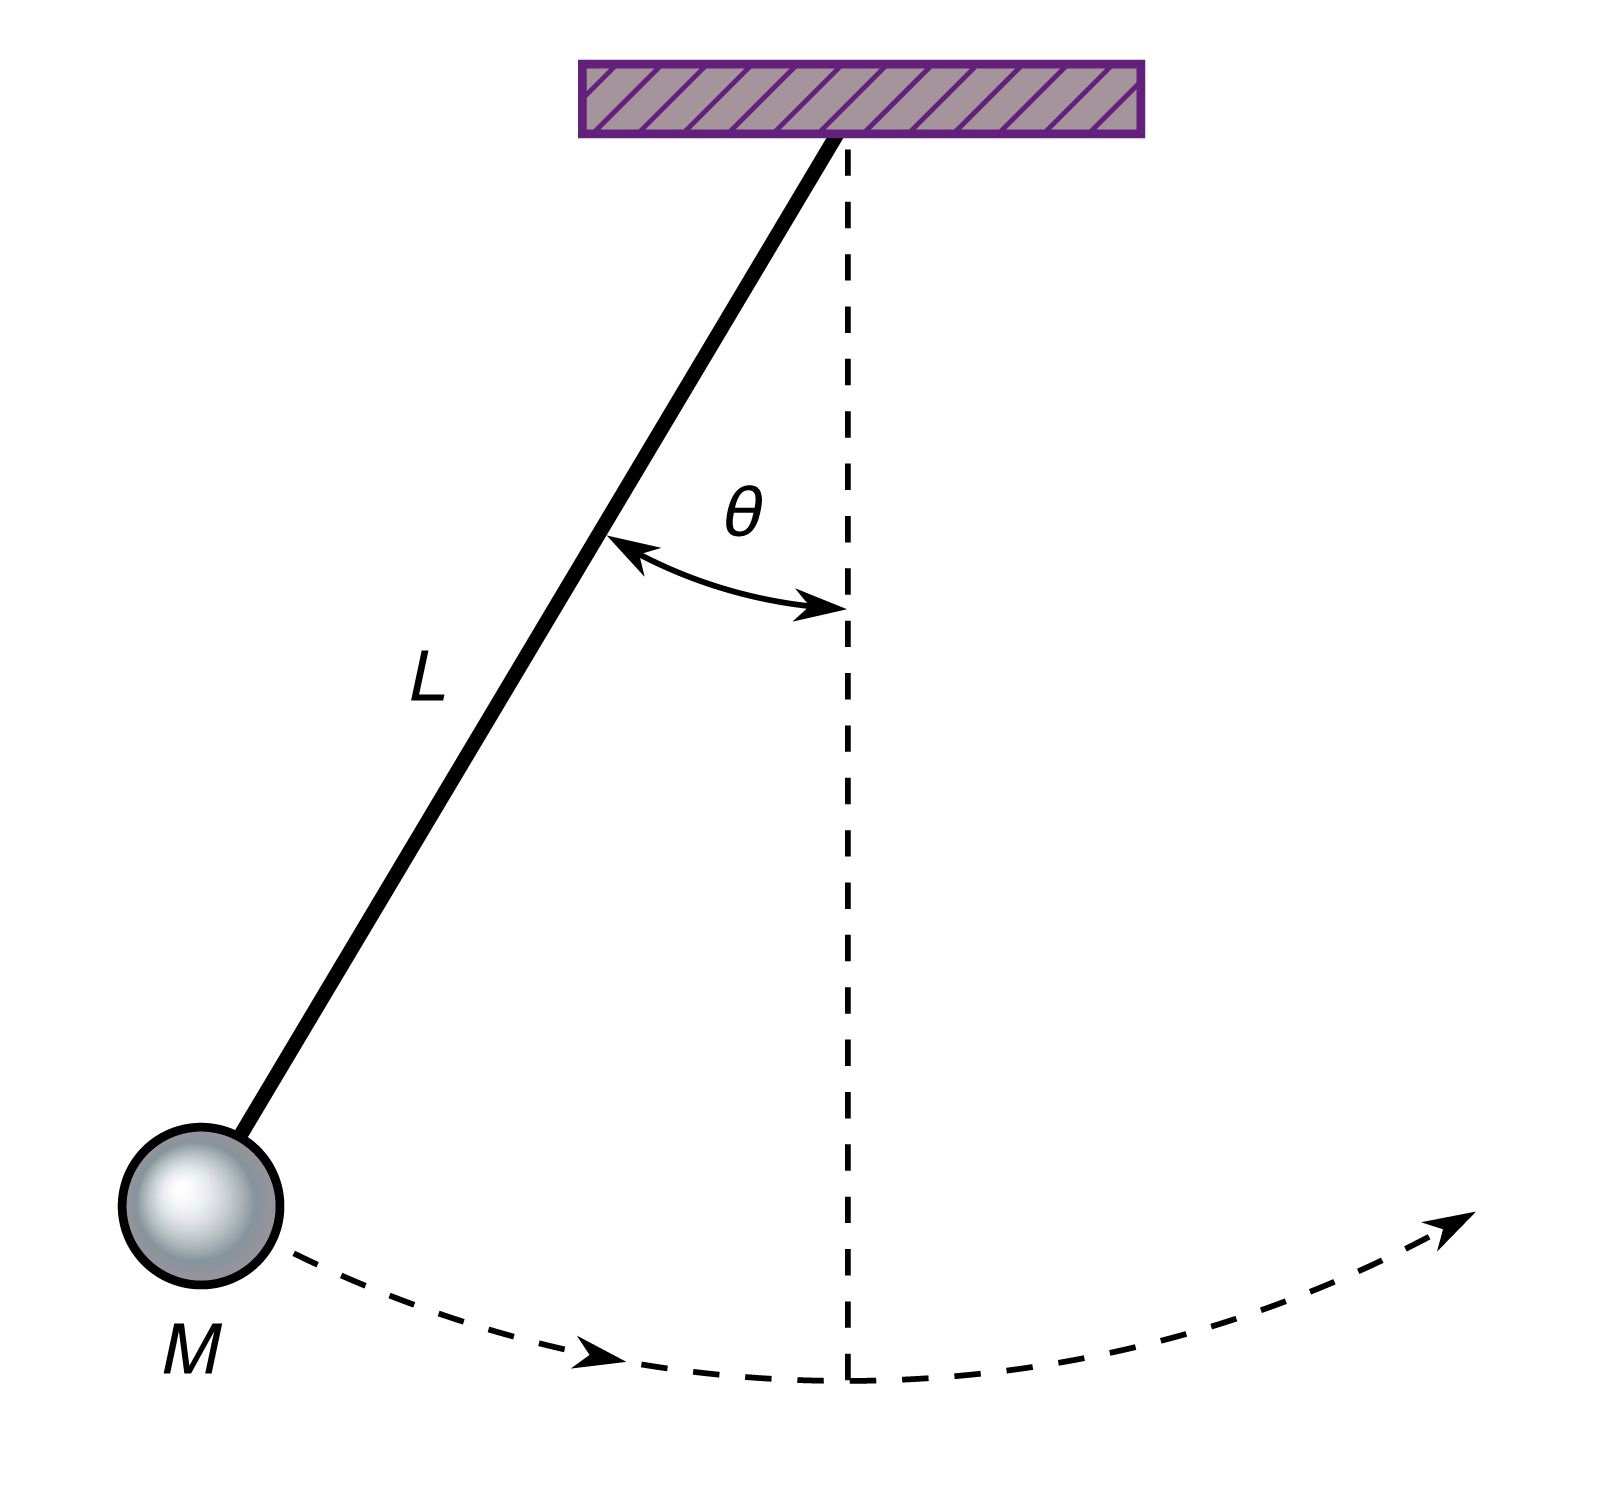
\includegraphics[scale=0.1]{IMG_0200.jpeg}	
		\end{center}
		
		
		
		\vfill
		
		
		
		corso A\\
		Università degli studi di Torino, Torino\\
		4 aprile 2024\\
		
		
	\end{center}
\end{titlepage}
\tableofcontents

\newpage
\textcolor{white}{.}
\vfill


\section{Scopo dell’esperienza}
\section{Premesse teoriche}
\section{Scelta strumento di misura}


\begin{table}
	\caption{Example of table with \texttt{tabularray}.}
	\label{tab:example}
	\centering
	\begin{tblr}{
			colspec={cccc},
			row{1}={font=\bfseries},
			column{1}={font=\itshape},
			row{even}={bg=gray!10},
		}
		& Cronometro analogico  & Cronometro digitale  &  Fotocellula   \\
		\toprule
		Model $X$ & X1 & X2 & X3  \\
		Model $Y$ & Y1 & Y2 & Y3  \\
		Model $Z$ & Z1 & Z2 & Z3  \\
		\bottomrule
	\end{tblr}
\end{table}



\section{Dipendenza dall’angolo}
\subsection{Fit lineare}
\subsection{Fit parabolico}
\subsection{g}

\section{Dipendenza dalla lunghezza}
\subsection{Fit lineare}
\subsection{Confronto parametri retta}

\section{Dipendenza dalla massa}


\section{Conclusioni}



\end{document}
